\section{Pacote Python e dez cenários adicionais}
\label{sec:package}
\subsection{Implementação pragmática e estimandos}
O pacote instalável \texttt{relative-dml}, versão 0.1.0, contém quatro classes. A interface comum usa \texttt{fit}, \texttt{predict\_ratio} e \texttt{predict\_lift}. Fixamos a convenção $\operatorname{lift}=R-1$; por exemplo, $R=1{,}2$ corresponde a lift de 20\%, não a 20 pontos percentuais. As covariáveis devem ser numéricas, finitas e anteriores ao tratamento. A primeira versão considera observações i.i.d.; não implementa inferência por clusters nem uma rotina de otimização comercial.

\texttt{DiscreteQLearner} aplica a identidade multiclasses de \cite{fuchs2026}, ajustando probabilidades de braço na população completa e entre conversores. \texttt{DiscreteDML} estima médias aumentadas por braço. Para $e_j(x)=\Pp(T=j\mid X=x)$, constrói fora do fold
\[
Z_j=\hat\mu_j(X)+\frac{\ind(T=j)}{\hat e_j(X)}\{Y-\hat\mu_j(X)\}.
\]
O resto exato é
\[
\E[Z_j\mid X]-\mu_j(X)
=\left(1-\frac{e_j(X)}{\hat e_j(X)}\right)\{\hat\mu_j(X)-\mu_j(X)\}.
\]
Cada sinal é regressado em $X$; só então formamos a razão das duas médias estimadas. A consistência da razão depende também da consistência das regressões finais e da positividade do denominador. Não dividimos sinais individuais nem cortamos seus valores negativos. Essa opção implementa a alternativa simples discutida após \eqref{eq:relloss}, sem atribuir dupla robustez exata à correção de Taylor do Apêndice~\ref{app:ratio}.

\texttt{ContinuousDML} encapsula o momento já utilizado em \texttt{experiments.py}, com três folds estratificados pelo outcome. A nuisance de baseline é uma classificação de $Y$ em $(X,T)$ avaliada na dose de referência; a média da dose é uma regressão de $T$ em $X$. A base implementada é $(t-t_{\rm ref})[1,V(x)]$, com modificadores $V$ pré-especificados e derivados de $X$. Sem modificadores, há apenas uma inclinação comum. A API não implementa as bases de splines nem o aprendiz de políticas estocásticas discutidos na teoria. Os erros-padrão dos coeficientes mantêm as condições de inferência da Seção~\ref{sec:dml}.

\subsection{Q contínuo por classificação de origens conjuntas}
\texttt{ContinuousQLearner} implementa uma variante simples da classificação de razões de densidade. Construímos uma origem $S=1$ com $(X,T)$ dos conversores e uma origem $S=0$ com $(X,T)$ da população completa. As origens recebem o mesmo peso total. Se $D(x,t)=\Pp(S=1\mid X=x,T=t)$ nessa mistura, então
\[
\frac{D(x,t)}{1-D(x,t)}
=\frac{f_{X,T\mid Y=1}(x,t)}{f_{X,T}(x,t)}
=\frac{\mu(t,x)}{\Pp(Y=1)}.
\]
Portanto, $\logit D(x,t)-\logit D(x,t_0)=\log R(t,t_0;x)$. A referência conjunta mantém a distribuição de alocação observada; a comparação de doses mantém $X$ fixo. Não é necessário simular doses de uma densidade condicional ajustada. O classificador recebe os registros positivos com peso $(n+n_1)/(2n_1)$ e todos os registros com peso $(n+n_1)/(2n)$, onde $n_1=\sum_iY_i$.

Conversores aparecem nas duas origens e não se tornam observações independentes adicionais. Uma eventual validação para tuning deve dividir os registros originais antes dessa duplicação. Esta é uma construção plug-in próxima de um S-learner: não há garantia DR nem alegação de vantagem estatística sobre regressão direta de outcome. Ela difere do Q de inclinação exponencial com densidade pré-fixada do primeiro Monte Carlo. Nas tabelas seguintes, ``Q'' designa a implementação discreta ou contínua correspondente ao cenário.

\subsection{Desenhos, protocolo e escolha do estágio final}
Mantemos $X_1\in\{-1,+1\}$ e $X_2\sim\operatorname{Unif}[-1,1]$, independentes. Nos novos desenhos,
\begin{equation}
\mu(t,x)=B\exp(0{,}65x_1+0{,}4x_2)
\exp\{t(\beta_0+\beta_1x_1)+\kappa t^2\}.
\label{eq:package-dgp}
\end{equation}
O padrão é $B=0{,}04$, $(\beta_0,\beta_1)=(-0{,}35,-0{,}20)$ e $\kappa=0$. No caso contínuo, usamos a densidade de \eqref{eq:simf}, agora com $\alpha(x)=c(0{,}9x_1+0{,}6x_2)$ e $c=1$. No discreto, $\Pp(T=j\mid X=x)=\exp\{j\alpha(x)\}/\sum_{\ell=0}^{K-1}\exp\{\ell\alpha(x)\}$, com braços $j=0,\ldots,K-1$.

Os seis casos contínuos são: efeito nulo ($\beta_0=\beta_1=0$); efeito comum ($\beta_1=0$); heterogêneo (padrão); conversão rara ($B=0{,}008$); pouco overlap ($c=4$); e curva omitida ($\kappa=0{,}8$). Os quatro discretos são: binário aleatorizado ($K=2,c=0$); binário confundido ($K=2,c=1$); três braços ($K=3,c=1$); e binário raro ($K=2,c=1,B=0{,}008$). As probabilidades de \eqref{eq:package-dgp} permanecem em $(0,1)$ nos suportes utilizados; o código também verifica essa condição em cada amostra. A conversão marginal varia por cenário, e não foi fixada em 6\%.

Comparamos Q, DML e um S-learner de conversão em $(X,T)$. As classificações e regressões de nuisance usam histogram gradient boosting com 100 iterações, taxa de aprendizagem 0,1, até oito folhas, pelo menos 50 registros por folha e regularização $L_2=2$. Desativamos early stopping para manter o protocolo explícito. No DML contínuo, $V(x)=x_1$ em todos os casos, inclusive nos efeitos nulo e comum; o ajuste não recebe antecipadamente a informação de que a heterogeneidade é zero. A forma relativa linear favorece esse estimador quando é correta, enquanto Q e S usam classes flexíveis: esta comparação não isola exclusivamente o benefício da ortogonalidade.

Uma rodada piloto de 30 replicações por cenário, semente 20260906, revelou instabilidade na regressão final discreta quando utilizava os mesmos parâmetros das nuisances: houve clipping em todas as 30 replicações de cada caso discreto. Os resultados completos dessa rodada foram preservados em \texttt{results/pilot}. Em resposta, fixamos apenas para o estágio final do DML discreto 30 iterações, taxa de aprendizagem 0,05, até quatro folhas, mínimo de 200 registros por folha e $L_2=10$. Isso regulariza sinais AIPW ruidosos sem substituir o estimando ou truncar os sinais individuais. Os demais modelos ficaram fixos.

A avaliação principal abaixo usa novas sementes, com base 20270906. Para cada cenário e replicação, geramos $n=12\,000$ registros de treino e outros $n_{\rm test}=2\,000$ independentes para avaliação; são 30 replicações por cenário e 900 ajustes, além dos 900 ajustes do piloto. A API de DML usa três folds. No contínuo, avaliamos $t\in\{-0{,}8,-0{,}4,0{,}4,0{,}8\}$ contra zero; no discreto, cada braço não controle contra o braço zero. A verdade é calculada diretamente por \eqref{eq:package-dgp}. Novas sementes separam a avaliação dos dados usados para alterar o estágio final, mas os dez desenhos continuam sendo os mesmos; não se trata de seleção cega de desenhos ou benchmark exaustivo.

\subsection{Métricas e resultados executados}
A métrica principal por replicação é
\[
\operatorname{RMSE}_{\log R}
=\left\{\frac{1}{n_{\rm test}|\mathcal C|}
\sum_{i=1}^{n_{\rm test}}\sum_{t\in\mathcal C}
\big[\log\widehat R(t,0;X_i)-\log R(t,0;X_i)\big]^2\right\}^{1/2}.
\]
Reportamos a média dessa métrica entre replicações; seu erro Monte Carlo é o desvio-padrão das 30 métricas dividido por $\sqrt{30}$. A segunda métrica é o erro absoluto médio do lift, $\E_{\rm teste}|\widehat R-R|$, também calculado por replicação. Um erro de 0,1 corresponde a dez pontos percentuais \emph{na escala do lift relativo}, não na probabilidade de conversão. Os arquivos brutos incluem ainda viés médio do lift, correlação de Spearman na maior dose comparada, contagem de conversores e mensagens de falha e clipping. Spearman fica indefinida para efeito verdadeiro constante.

\begin{table}[htbp]
\centering
\caption{Avaliação principal: média do RMSE de log-ratio e erro Monte Carlo entre parênteses. Trinta replicações, $n=12\,000$ e $n_{\rm test}=2\,000$ por cenário.}
\label{tab:scenarios-log}
\footnotesize
\setlength{\tabcolsep}{4pt}
\begin{tabular}{lrrrr}
\toprule
Cenário & Conv. (\%) & Q & DML & S-learner \\
\midrule
Contínuo: efeito nulo & 4.93 & 0.472 (0.017) & 0.067 (0.006) & 0.370 (0.014) \\
Contínuo: efeito comum & 4.79 & 0.431 (0.026) & 0.076 (0.010) & 0.356 (0.016) \\
Contínuo: heterogêneo & 4.61 & 0.460 (0.020) & 0.079 (0.010) & 0.377 (0.016) \\
Contínuo: conversão rara & 0.94 & 1.064 (0.057) & 0.185 (0.021) & 0.680 (0.038) \\
Contínuo: pouco overlap & 3.88 & 0.564 (0.029) & 0.126 (0.012) & 0.387 (0.018) \\
Contínuo: curva omitida & 6.29 & 0.413 (0.015) & 0.395 (0.003) & 0.333 (0.012) \\
Binário: aleatorizado & 4.07 & 0.462 (0.010) & 0.220 (0.008) & 0.276 (0.010) \\
Binário: confundido & 3.82 & 0.479 (0.012) & 0.273 (0.011) & 0.290 (0.011) \\
Discreto: três braços & 2.84 & 0.699 (0.019) & 0.545 (0.026) & 0.358 (0.009) \\
Binário: conversão rara & 0.72 & 0.896 (0.019) & 0.653 (0.029) & 0.514 (0.027) \\
\bottomrule
\end{tabular}

\end{table}

\begin{table}[htbp]
\centering
\caption{Erro absoluto médio do lift relativo; erro Monte Carlo entre parênteses. Mesmo protocolo da Tabela~\ref{tab:scenarios-log}.}
\label{tab:scenarios-lift}
\footnotesize
\setlength{\tabcolsep}{4pt}
\begin{tabular}{lrrrr}
\toprule
Cenário & Conv. (\%) & Q & DML & S-learner \\
\midrule
Contínuo: efeito nulo & 4.93 & 0.349 (0.022) & 0.055 (0.005) & 0.290 (0.014) \\
Contínuo: efeito comum & 4.79 & 0.323 (0.020) & 0.066 (0.009) & 0.292 (0.013) \\
Contínuo: heterogêneo & 4.61 & 0.369 (0.033) & 0.068 (0.008) & 0.319 (0.022) \\
Contínuo: conversão rara & 0.94 & 1.107 (0.234) & 0.161 (0.018) & 0.619 (0.069) \\
Contínuo: pouco overlap & 3.88 & 0.484 (0.038) & 0.114 (0.011) & 0.313 (0.016) \\
Contínuo: curva omitida & 6.29 & 0.515 (0.036) & 0.430 (0.002) & 0.394 (0.016) \\
Binário: aleatorizado & 4.07 & 0.285 (0.010) & 0.123 (0.006) & 0.153 (0.008) \\
Binário: confundido & 3.82 & 0.311 (0.014) & 0.161 (0.008) & 0.171 (0.010) \\
Discreto: três braços & 2.84 & 0.402 (0.019) & 0.316 (0.042) & 0.173 (0.005) \\
Binário: conversão rara & 0.72 & 1.036 (0.062) & 0.411 (0.024) & 0.326 (0.029) \\
\bottomrule
\end{tabular}

\end{table}

No caso contínuo heterogêneo, o RMSE médio de log-ratio foi 0.079 para DML, 0.460 para Q e 0.377 para S-learner. O DML utiliza aqui a forma relativa correta e apenas dois coeficientes. Seu RMSE aumenta para 0.185 com conversão rara e 0.126 com pouco overlap. Quando se omite curvatura verdadeira, o RMSE do DML chega a 0.395, enquanto o S-learner obtém 0.333. A restrição multiplicativa ajuda nos desenhos que a satisfazem e se torna uma fonte de erro no desenho curvo.

No binário aleatorizado, o DML com estágio final regularizado apresenta RMSE 0.220, frente a 0.462 do Q e 0.276 do S-learner. Essa regularização não resolve todos os regimes: com três braços, os RMSEs de DML e S-learner são 0.545 e 0.358; no binário raro, são 0.653 e 0.514. O S-learner é portanto uma referência relevante, e a garantia de consistência DR não implica menor erro em amostras finitas.

Foram concluídos 900 dos 900 ajustes principais; 0 falhas foram registradas. O DML discreto ainda apresentou clipping em 7/30 replicações com três braços e 8/30 no binário raro. A ausência de avisos no Q não garante precisão: seus erros nos desenhos raros permanecem grandes. As diferenças observadas dependem destes desenhos, classes e parâmetros; não sustentam superioridade geral de uma família.


\begin{figure}[htbp]
\centering
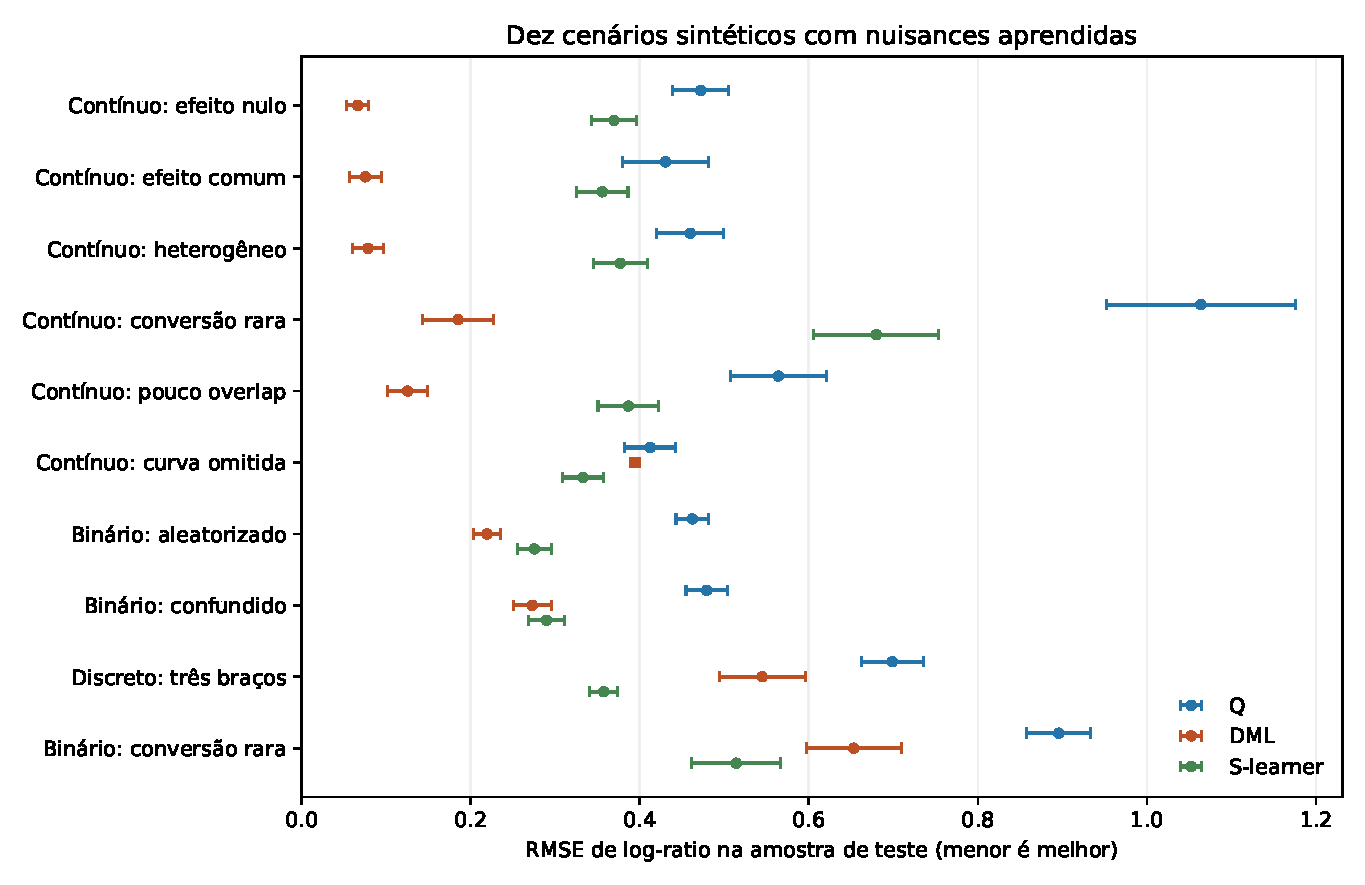
\includegraphics[width=\linewidth]{figures/scenario_comparison.pdf}
\caption{RMSE de log-ratio na amostra independente de teste. As barras são $1{,}96$ vezes o erro Monte Carlo da média das métricas, não intervalos para o efeito de um indivíduo.}
\label{fig:scenarios}
\end{figure}

\subsection{Estabilização, limites e reprodução}
O piso de propensão e de probabilidades usadas nas razões é 0,001. No DML discreto, somente as respostas \emph{após} a regressão final são limitadas a $[0{,}001,1]$; os sinais AIPW podem permanecer negativos. No S-learner, aplicamos o mesmo piso de resposta na avaliação. No Q contínuo, limitamos a probabilidade de origem a $[0{,}001,0{,}999]$; no Q discreto, aplicamos o piso às probabilidades de braço. Esses mecanismos são explicitamente distintos e não tornam iguais as classes de modelos. Um piso fixo pode alterar o alvo efetivo em regiões de baixa conversão ou overlap; resultados com clipping exigem análise de sensibilidade.

\begin{table}[htbp]
\centering
\caption{Replicações com ao menos um aviso de clipping, por cenário e método, na avaliação principal. O numerador conta ajustes, não indivíduos.}
\label{tab:scenarios-clipping}
\small
\begin{tabular}{lrrr}
\toprule
Cenário & Q & DML & S-learner \\
\midrule
Contínuo: efeito nulo & 0/30 & 0/30 & 0/30 \\
Contínuo: efeito comum & 0/30 & 0/30 & 0/30 \\
Contínuo: heterogêneo & 0/30 & 0/30 & 0/30 \\
Contínuo: conversão rara & 0/30 & 0/30 & 20/30 \\
Contínuo: pouco overlap & 0/30 & 0/30 & 0/30 \\
Contínuo: curva omitida & 0/30 & 0/30 & 0/30 \\
Binário: aleatorizado & 0/30 & 0/30 & 0/30 \\
Binário: confundido & 0/30 & 0/30 & 0/30 \\
Discreto: três braços & 0/30 & 7/30 & 0/30 \\
Binário: conversão rara & 0/30 & 8/30 & 21/30 \\
\bottomrule
\end{tabular}

\end{table}

O teste de curvatura é uma falsificação da forma relativa linear, não uma falha das identidades de Bayes ou do resto DR sob seu modelo correto. O caso de pouco overlap ainda tem densidade positiva em todo $[-1,1]$, mas atribui pouca informação a algumas comparações; nenhuma restrição de intervalo global verifica suporte condicional. A conversão rara reduz informação para todos os métodos. As tabelas não demonstram cobertura de intervalos de confiança nem consistência assintótica a partir de uma única dimensão amostral.

\texttt{scenario\_experiments.py} gera os dados e os CSVs; \texttt{make\_scenario\_figures.py} produz automaticamente as duas tabelas de métricas, a tabela de avisos e a figura a partir desses CSVs. Metadados registram versões efetivamente usadas, sementes e parâmetros. A rodada piloto pode ser reproduzida com \texttt{--seed 20260906 --pilot-final}; a avaliação principal usa a semente padrão 20270906. O pacote possui testes de identidades em populações finitas, braço multiclasses, referência não nula, recuperação de heterogeneidade e exclusão dos registros de treino nas predições de nuisance. Esses testes complementam o Monte Carlo, sem substituir validação em dados reais.
